\documentclass[fleqn]{homework}

\student{Stephen Brennan (smb196)}
\course{EECS 440}
\assignment{Programming 3}
\duedate{October 29, 2015}

\usepackage{hyperref}
%\usepackage{mathtools}
%\usepackage{graphicx}

\begin{document}
  \maketitle

  \section{Implementation Commentary}

  \subsection{Na\"{i}ve Bayes}

  The implementation of Na\"{i}ve Bayes is fairly straightforward compared to
  the artificial neural networks of the previous assignment.  The training phase
  is especially so.  I didn't encounter any issues with this implementation.

  \subsection{Logistic Regression}

  The implementation of logistic regression was only slightly more difficult
  than the Na\"ive Bayes implementation.  In this, we were required to minimize
  the loss function:

  \begin{equation}
    L(\vec{w},b) = \frac{1}{2} \lambda ||\vec{w}||^2 + \sum_{i} \log \left(1 + e^{-y_i(\vec{w}\cdot\vec{x} + b)}\right)
  \end{equation}

  I computed the following partial derivative (for each $w_j$):

  \begin{equation}
    \frac{\partial L}{\partial w_J} = \lambda w_j + \sum_{i} \frac{1}{1 + e^{y_i(\vec{w}\cdot\vec{x_i} + b)}} (-y_i x_{ij})
  \end{equation}

  And this partial derivative for $b$:

  \begin{equation}
    \frac{\partial L}{\partial b} = \sum_{i} \frac{1}{1 + e^{y_i(\vec{w}\cdot\vec{x_i} + b)}} (-y_i)
  \end{equation}

  Initially, I tried implementing my own gradient descent.  However, after much
  fiddling of the step size and termination conditions without successful
  results, I decided that I should use a NumPy/SciPy minimization routine.  I
  implemented both the loss function and the gradient as Python functions, and
  used the \texttt{scipy.optimize.minimize} function.  This is actually a
  gateway to a number of different minimization algorithms.  I tried three:
  ``CG'', ``BFGS'', and ``Netwon-CG'' (documented with references in
  \href{https://docs.scipy.org/doc/scipy/reference/generated/scipy.optimize.minimize.html}{SciPy's
    documentation}).  I discovered that all except ``Newton-CG'' gave strange
  errors and floating point overflow messages, so I stuck with ``Newton-CG''.

  \subsection{Internal Cross Validation}

  I was able to implement internal cross validation very simply.  I wrote a
  generic \texttt{internal\_cross\_validation()} function that trains and tests
  a classifier for each parameter value in a range, using 5-fold validation.  It
  chooses the best parameter value using any statistic you'd like (I use AUC
  throughout) and returns it.  Since the function just takes the class name of
  the classifier, I was able to add in internal cross validation through a
  single function call in both classifiers' \texttt{fit()} methods.

  \subsection{Command Line Interface}

  I made some modifications to the command line interface (as mentioned in an
  email conversation).  However, these make \textit{no impact} on the prescribed
  behavior in the assignment.

  \begin{itemize}
  \item The command line parameter \texttt{--m\_value [n]} can specify the
    parameter \texttt{m} for the \texttt{NaiveBayes} classifier.  If
    unspecified, \texttt{m} takes a value of \texttt{None}, which causes the
    classifier to use internal cross validation (as expected).
  \item Similarly, the command line parameter \texttt{--lambda} defaults to
    \texttt{None} instead of the number it defaulted to before.  This will
    trigger internal cross validation (as required by the assignment).  However,
    you can also override internal cross validation by providing
    \texttt{--lambda [n]} on the command line.
  \end{itemize}

  \section{Questions}

  \begin{problem}{a}
    \begin{question}
      What is the accuracy of Na\"ive Bayes and logistic regression on the
      different learning problems?  For each problem, perform a $t$ test to
      determine if either is superior with 95\% confidence.
    \end{question}

    The following table summarizes one run of 5-fold cross validation on each
    combination of dataset and algorithm.

    \vspace{0.3cm}
    \begin{tabular}{rrr}
      \hline
      Dataset & Na\"ive Bayes & Logistic Regression \\
      \hline
      Voting & 0.968 (0.026) & 0.986 (0.005) \\
      Spam & 0.705 (0.006) & 0.706 (0.002) \\
      Volcanoes & 0.633 (0.016) & 0.734 (0.020) \\
      \hline
    \end{tabular}
    \vspace{0.3cm}

    Since the data above were not gathered using the same folds, we must perform
    an independent two-sample $t$ test (rather than the dependent one presented
    in the slides).  The $t$ test requires the use of the corrected sample
    standard deviation, while the values given above are uncorrected.  The
    difference being that corrected sample standard deviation has the following
    formula:

    \begin{equation}
      s = \sqrt{\frac{1}{n-1} \sum_{i=1}^n (x_i - \bar{x})^2}
    \end{equation}

    While the uncorrected standard deviation (presented in the table above) has
    the formula:

    \begin{equation}
      s = \sqrt{\frac{1}{n} \sum_{i=1}^n (x_i - \bar{x})^2}
    \end{equation}

    To correct this. we multiply each standard deviation by
    $\sqrt{\frac{n}{n-1}} = \sqrt{\frac{5}{4}}$ to obtain the $s$ test
    statistic.  The corrected values of $s$ are presented in the table below:

    \vspace{0.3cm}
    \begin{tabular}{rrr}
      \hline
      Dataset & Na\"ive Bayes & Logistic Regression \\
      \hline
      Voting & 0.0291 & 0.0058 \\
      Spam & 0.0067 & 0.0022 \\
      Volcanoes & 0.0179 & 0.0224 \\
      \hline
    \end{tabular}
    \vspace{0.3cm}

    To compute the 95\% confidence interval for the difference between the
    accuracy of na\"ive Bayes and logistic regression, we compute
    $Acc_{NB} - Acc_{LR} \pm t_{95\%,2n-2} \sqrt{s_{NB}^2 + s_{LR}^2} *
    \sqrt{\frac{1}{n}}$,
    where $n$ is the number of folds, which is 5.  Also, $t_{95\%,8} = 2.306$.
    The confidence intervals are presented in the table below:

    \vspace{0.3cm}
    \begin{tabular}{rl}
      \hline
      Dataset & Confidence Interval \\
      \hline
      Voting & $0.968 - 0.986 \pm 2.306 * 0.013 \to [-0.049, +0.013]$ \\
      Spam & $0.705 - 0.706 \pm 2.306 * 0.003 \to [-0.008, +0.006]$ \\
      Volcanoes & $0.633 - 0.734 \pm 2.306 * 0.013 \to [-0.131, -0.071]$ \\
      \hline
    \end{tabular}
    \vspace{0.3cm}

    Since 0 is only \textbf{not} contained in the confidence interval for
    Volcanoes, we can only reject the null hypothesis (that both algorithms
    perform the same) on Volcanoes.  This shows that Logistic Regression is
    probably better for Volcanoes than Na\"ive Bayes.

  \end{problem}

  \begin{problem}{b}
    \begin{question}
      Compare these two methods with your previously implemented methods (trees,
      perceptrons, ANNs).  Discuss which, if any, seems to be better on the
      provided learning problems in terms of (i) accuracy, precision, recall,
      and the area under ROC, (ii) runtime, and (iii) code complexity and
      difficulty of implementation.  Note that this question is about
      \textit{general trends}--it may not happen that any one algorithm will
      turn out to be superior across all problems (cf. the NFL theorem).  So use
      your judgment to determine ``betterness.''  For methods that appear about
      equal in terms of accuracy, look at the precision and recall and try to
      explain any patterns you see.
    \end{question}
  \end{problem}

  The following table presents an overview the best results I have presented for
  each previously implemented method, on the \texttt{voting} dataset.  Plus or
  minus values are standard deviations, not confidence intervals.

  \vspace{0.3cm}
  \begin{tabular}{rrrrr}
    \hline
    Classifier & Accuracy & Precision & Recall & AUC \\
    \hline
    Decision Tree & 0.984 & * & * & * \\
    Perceptron & 0.986 $\pm$ 0.009 & 0.995 $\pm$ 0.010 & 0.974 $\pm$ 0.016 & 0.994 \\
    ANN & * & * & * & 0.994 \\
    Na\"ive Bayes & 0.968 $\pm$ 0.026 & 0.975 $\pm$ 0.026 & 0.955 $\pm$ 0.066 & 0.967 \\
    Logistic Regression & 0.986 $\pm$ 0.005 & 0.990 $\pm$ 0.012 & 0.980 $\pm$ 0.019 & 0.997 \\
    \hline
  \end{tabular}
  \vspace{0.3cm}

  Looking at the results above, I don't think it's fair to make any
  generalizations about which classifier is best.  The numbers are so close that
  none of them can really be called significant (even the precision and recall).
  In terms of runtime, the decision tree, and na\"ive Bayes classifier were
  always pretty much instantaneous in training.  Logistic regression is a bit
  slower, along with perceptron.  Finally came the ANN.

  The following table presents an overview of the best results I have presented
  for each previously implemented method, on the \texttt{spam} dataset.

  \vspace{0.3cm}
  \begin{tabular}{rrrrr}
    \hline
    Classifier & Accuracy & Precision & Recall & AUC \\
    \hline
    Decision Tree & 0.643 & * & * & * \\
    Perceptron & 0.663 $\pm$ 0.013 & 0.632 $\pm$ 0.011 & 0.991 $\pm$ 0.012 & 0.525 \\
    ANN & * & * & * & 0.508 \\
    Na\"ive Bayes & 0.705 $\pm$ 0.006 & 0.743 $\pm$ 0.003 & 0.807 $\pm$ 0.009 & 0.753 \\
    Logistic Regression & 0.706 $\pm$ 0.002 & 0.728 $\pm$ 0.003 & 0.848 $\pm$ 0.002 & 0.742 \\
    \hline
  \end{tabular}
  \vspace{0.3cm}

  I think it's fair to say that on \texttt{spam}, na\"ive Bayes and logistic
  regression are both markedly better than the alternatives.  Between the two,
  logistic regression has worse precision at the expense of better recall,
  indicating that it probably selects more false positives, which is reflected
  in the AUC.  Since false positives are a bad thing in the world of spam
  detection, it would make sense that na\"ive Bayes would be preferred for its
  fewer false positive.

  In terms of runtime, ANN performed the worst by far (due to the huge amount of
  examples).  Decision trees were probably next worst, followed by the single
  perceptron.  Logistic regression was probably second best, and na\"ive Bayes
  again was fastest (especially when you do not do internal cross validation).

  Finally, the available data on \texttt{volcanoes} is presented below for each
  classifier.

  \vspace{0.3cm}
  \begin{tabular}{rrrrr}
    \hline
    Classifier & Accuracy & Precision & Recall & AUC \\
    \hline
    Decision Tree & 0.674 & * & * & * \\
    Perceptron & 0.806 $\pm$ 0.051 & 0.760 $\pm$ 0.063 & 0.635 $\pm$ 0.252 & 0.719 \\
    ANN & * & * & * & 0.758 \\
    Na\"ive Bayes & 0.633 $\pm$ 0.016 & 0.466 $\pm$ 0.013 & 0.826 $\pm$ 0.021 & 0.725 \\
    Logistic Regression & 0.734 $\pm$ 0.020 & 0.624 $\pm$ 0.040 & 0.473 $\pm$ 0.032 & 0.705 \\
    \hline
  \end{tabular}
  \vspace{0.3cm}

  Not too surprisingly, the ANN and perceptron displayed the best performance
  here.  While the accuracy, precision, and recall data are not available for
  the ANN, it does show the best AUC.  Next comes the perceptron, followed by
  logistic regression, decision tree, and finally na\"ive Bayes.  It is not
  surprising that na\"ive Bayes performs the worst -- it assumes that the
  features are independent, when clearly the individual pixels of volcano image
  must be interpreted together in order to provide insight.  This is probably
  why the ANN performed well on it.

  However, in terms of runtime, ANN was still far and away the worst, along with
  the perceptron.  If you enable internal cross validation, na\"ive Bayes and
  logistic regression come next, followed by the decision tree.  However, I
  would say that na\"ive Bayes and logistic regression perform better without
  internal cross validation.

  The implementation difficulty can be assessed independently of the dataset.  I
  must admit that na\"ive Bayes was the easiest to implement -- taking only an
  hour or two, with very few issues to address after implementation.  I would
  say that the next easiest was decision trees, which had an intuitive and
  elegant recursive structure that made them nice to implement (but rather
  inefficient).  Logistic regression came next, since it required computing
  gradients and minimizing functions, which is considerably more difficult than
  recording frequencies as in na\"ive Bayes.  Finally, without a shadow of a
  doubt, artificial neural networks were the most difficult.  Manipulating many
  large matrices of parameters of arbitrary size was very difficult, and the
  gradient computations took hours to get right on their own.

  \begin{problem}{c}
    \begin{question}
      Plot the choices of $m$ and $\lambda$ for the different folds and datasets
      on a graph with the datasets on the x-axis, the average choice on the
      y-axis with max and min values indicating the max and min choices on that
      dataset.  Use a log-scale for the y-axis.  Discuss what these choices
      imply about the data and the algorithms.
    \end{question}

    The parameter choices for $m$ in na\"ive Bayes are plotted below:

    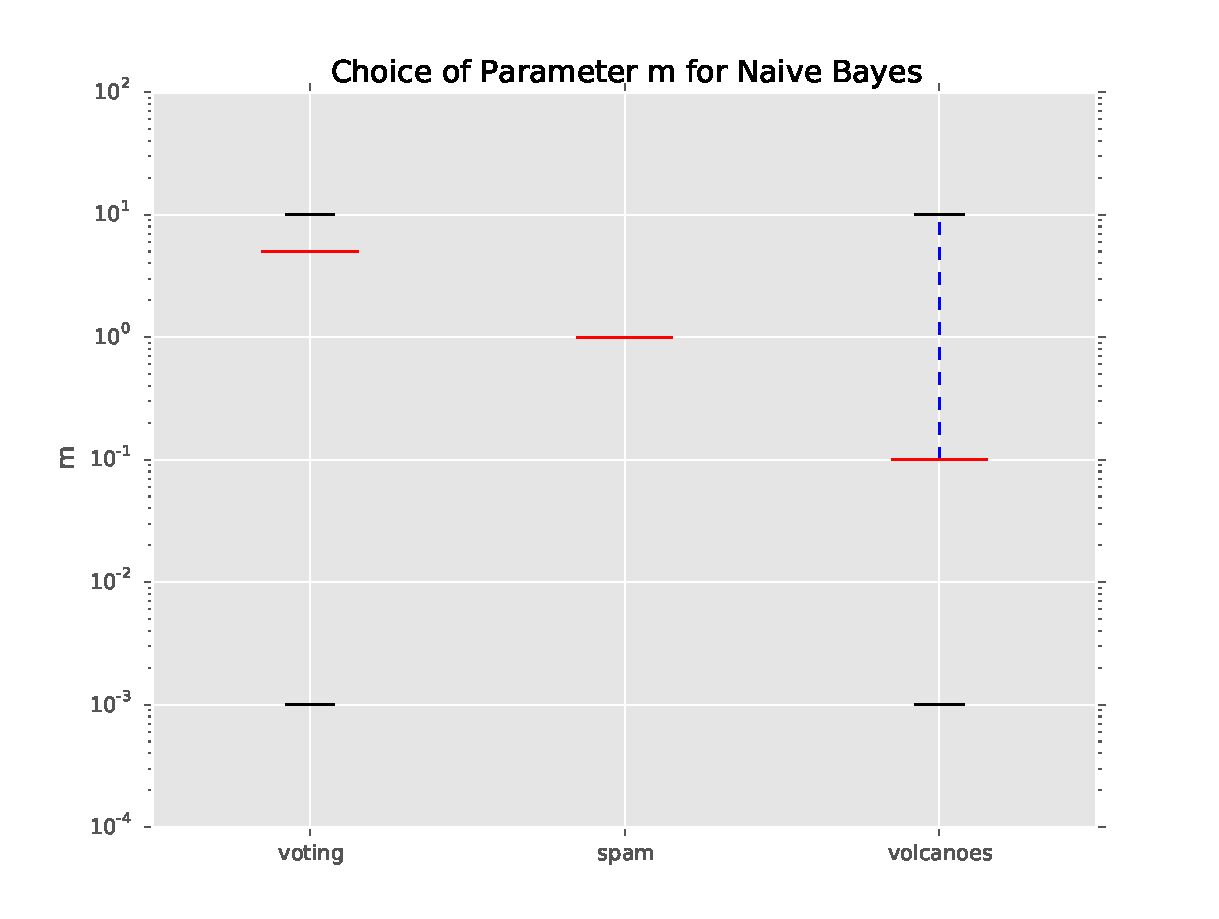
\includegraphics[width=0.8\textwidth]{nbayes_m.pdf}

    It's worth noting that for voting, one of the folds chose $m=0$.  For any
    folds where a parameter was 0, I removed those instances (since the minimum
    couldn't be displayed).  The only dataset that had a notably consistent
    choice of parameter was spam, which always chose 1.  The others chose values
    less than or equal to 10, meaning that they didn't put very high emphasis on
    the prior ``knowledge'' that each of the conditional probabilities were
    equal.

    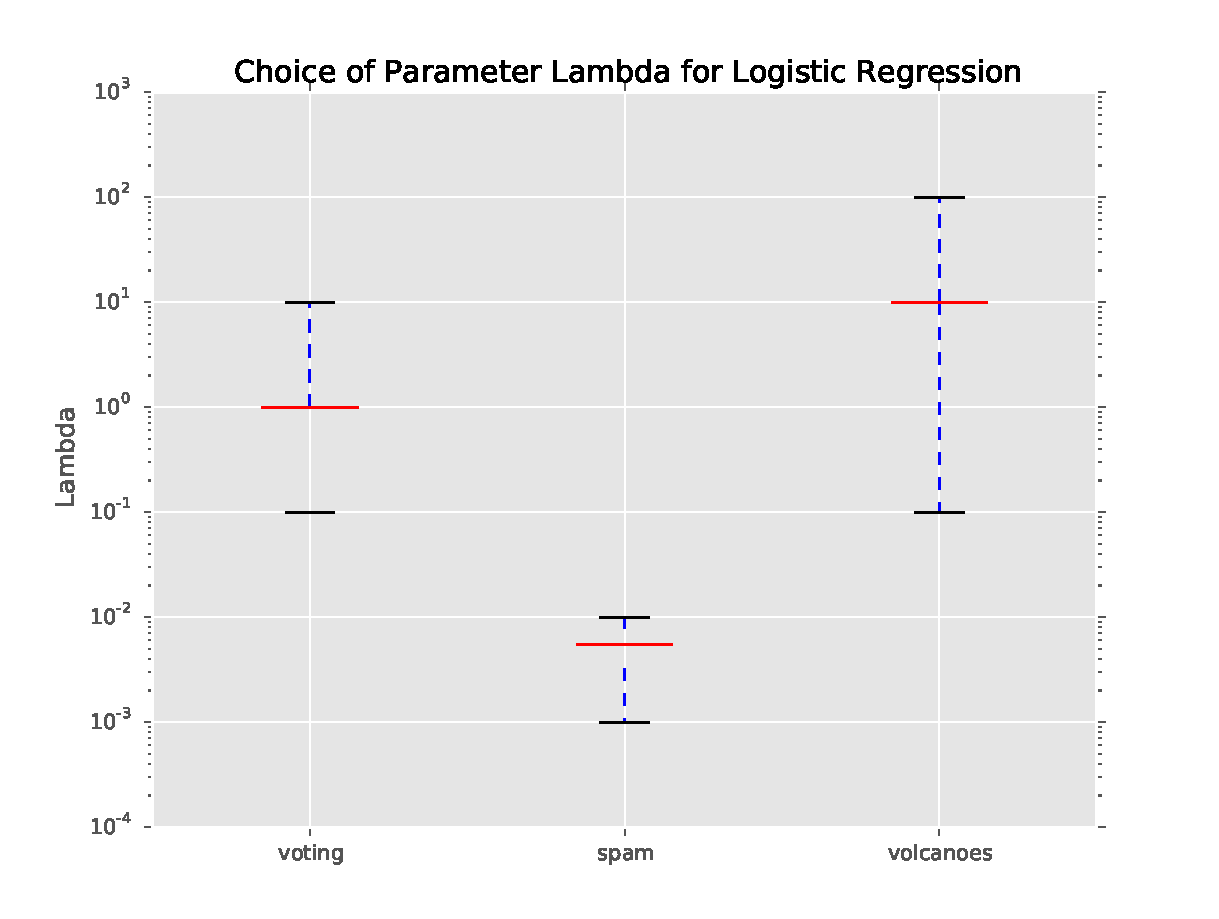
\includegraphics[width=0.8\textwidth]{logreg_lambda.pdf}

    Since $\lambda$ was the coefficient of the weight penalty term, it follows
    that lower choices for $\lambda$ correspond to datasets that require more
    complex models.  Spam here had clearly the lowest choices of $\lambda$,
    including three folds where $\lambda=0$, which could not be plotted here.

    In other words, the plots for both $m$ and $\lambda$ seem to imply that spam
    was consistently a complex problem that required more complex models, and
    thus less emphasis on prior knowledge or small weights.
    
  \end{problem}

  \begin{problem}{d}
    \begin{question}
      Compare the performance of the tuned classifiers with the MLE classifiers.
      Do you notice a benefit to tuning the parameters in this way?
    \end{question}

    I assume the meaning of this question is internal cross validation versus
    just setting the parameter of interest to 0.  Below, I've recorded
    performance information for na\"ive Bayes with $m=0$.

    \vspace{0.3cm}
    \begin{tabular}{rrrrr}
      \hline
      Dataset & Accuracy & Precision & Recall & AUC \\
      \hline
      Voting & 0.984 $\pm$ 0.012 & 0.985 $\pm$ 0.020 & 0.979 $\pm$ 0.010 & 0.994 \\
      Spam & 0.705 $\pm$ 0.003 & 0.743 $\pm$ 0.002 & 0.808 $\pm$ 0.005 & 0.751 \\
      Volcanoes & 0.645 $\pm$ 0.019 & 0.473 $\pm$ 0.019 & 0.758 $\pm$ 0.049 & 0.703 \\
      \hline
    \end{tabular}
    \vspace{0.3cm}

    The MLE classifier has a better performance in every statistic for voting,
    nearly identical for spam, and split for volcanoes.  I wouldn't say that I
    see a benefit to the tuned parameters in this case.

    Below is the performance for the classifier for logistic regression with
    $\lambda=0$.

    \vspace{0.3cm}
    \begin{tabular}{rrrrr}
      \hline
      Dataset & Accuracy & Precision & Recall & AUC \\
      \hline
      Voting & 0.986 $\pm$ 0.013 & 0.985 $\pm$ 0.020 & 0.985 $\pm$ 0.021 & 0.985 \\
      Spam & 0.706 $\pm$ 0.004 & 0.728 $\pm$ 0.003 & 0.848 $\pm$ 0.003 & 0.742 \\
      Volcanoes & 0.740 $\pm$ 0.009 & 0.639 $\pm$ 0.021 & 0.482 $\pm$ 0.053 & 0.703 \\
      \hline
    \end{tabular}
    \vspace{0.3cm}

    Voting performs moderately better tuned, spam displays no difference at all,
    and volcanoes also performs moderately better tuned.  In this case, there
    may be a very small benefit to tuning (which also seems to echo the
    parameter choices in the graph above).
  \end{problem}

\end{document}